%This section provides details on other projects/publications which are in the similar fields.

Mining structured information from unstructured text documents has recently gained attention.
Current approaches are still far from an fully automated and completely accurate processing.
However, the challenge has led to a number of research and applications.
Each work focused on solving a particular problem in the big pictures with regard to some specific languages. 

This section provides an insight into other contributions to the mining problem.
Both research-oriented works and industry applications are taken into account.

% http://knowtator.sourceforge.net/
% http://knowtator.sourceforge.net/docs/Ogren_HLT-NAACL06_Demo_Abstract_Final.pdf
Knowtator is a general-purpose text annotation tool.
Developed by scientists at Division of Biomedical Informatics, 
it uses Protégé knowledge-base as the database.
As an early development of tool for annotating data, Knowtator has a number of limitations (OS dependent, no client-server, no automatic detection).
The remarkable feature of Knowtator is the ability to relate annotations to each other via the slot \textit{reference}.
The tool has been implemented as a Protégé plug-in for wider-spread usage.


%http://www.aclweb.org/anthology/N/N13/N13-3004.pdf
%Anafora: A Web-based General Purpose Annotation Tool

Anafora is an open source web-based text annotation tool,
developed by scientists of University of Colorado at Boulder.
It distinguishes itself from previous contribution in the field of OS platform.
Before the introduction of Anafora, old tools were written as a local application in a local machine under the threat of data fragmentation.
Anafora is a web-based tool with client-server structure. % OK, INTRODUCTION TO ANAFORA

\begin{figure}[!htb]
	\centering
	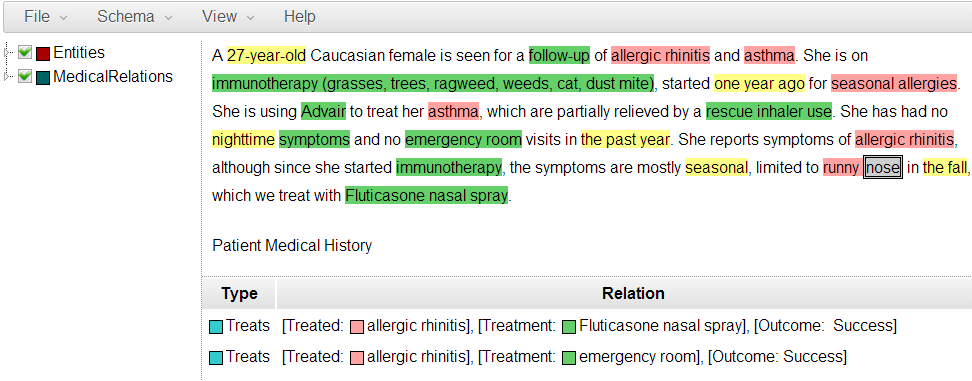
\includegraphics[width=\textwidth]{Images/anafora}
	\caption{Anafora graphics user interface}
	\label{fig:First}
\end{figure}


Anafora is designed for the medical domain with a medical named entity tags, not a general domain.
It is developed with a server in Django (a Python framework) and a client in jQuery (a JavaScript library).
Besides, it stores annotations in each single XML files.
By doing so, authors claim that the tool is agile and flexible.
The project hierachy is designed to be the file/directory structures.
The application provides an automatic detection of named entities.
Users can change/add details to the annotation by mouse or keyboard.
Anafora was designed for English.

The limitation of Anafora lies in the data structure.
Complicated definitions like relations (or relation properties) among entities are not supported.
It may be the trade-off when authors want to develop lightweight tools based on a simple data structure such as XML.

\comment{Ondrej}{XML can be complicated too}

% http://brat.nlplab.org/

BRAT rapid annotation tool is a web-based tool for text annotation,
most useful to add notes to existing text documents (taken from the introduction of BRAT).
It is developed by the University of Tokio.
This tool does support the linking relation between two entities and even the link from entities to a definition outside documents (such as Wikipedia).

\begin{figure}[!htb]
	\centering
	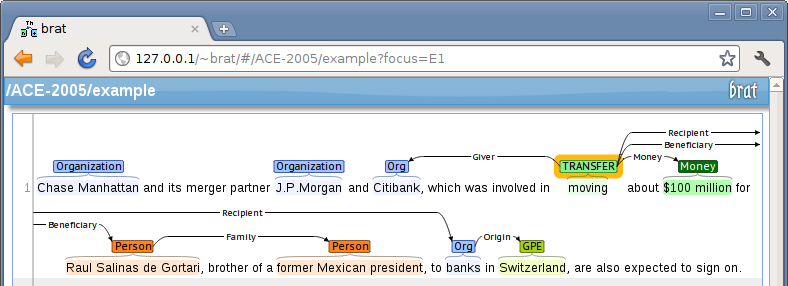
\includegraphics[width=\textwidth]{Images/brat}
	\caption{BRAT graphics user interface}
	\label{fig:Second}
\end{figure}

The strong point of BRAT is the simplicity of usage.
The tool offers a comprehensive visualization with mouse-based activities,
a method for linking to an external resources (such as Freebase, Wikipedia, and Open Biomedical Ontologies).
A number of other useful functions are \textit{save, export from standoff format, search}.
The brat \comment{Ondrej}{BRAT?} standoff format is a simple format developed for the visualization of the tool,
in which data is stored in two files: a text file \textit{.txt} and an annotation file \textit{.ann}.

The weak point of the tool is that it does not support any automatic recognition of entities.
All annotations have to be done manually.
This leads to a feature that the tool could be applied on a wide range of languages.
However, the limitation leads to a fact that BRAT is merely an editor for annotating.
